% $Id: Note_ResFit_QCDMC.tex,v 1.5 2010/07/24 21:31:30 mschrode Exp $


\subsection{Effects from additional jet activity}\label{sec:ResFit:QCDMC:AddJetAct}

One assumption of the maximum likelihood method is the \pt balance on
particle level of the two leading jets in each dijet event.
In realistic QCD events, however, additional jets, e.g. from hard
gluon radiation, cause a \ptparticle imbalance.
The resolution measurement, therefore, will be biased
towards larger values.
The effect is demonstrated in Fig.~\ref{fig:ResFit:QCDMC:AddJetAct:Fit}: 
The Gaussian resolution $\sigma$ ~\eqref{eq:ResFit:ToyMC:Sigma} is derived using the maximum
likelihood fit.
As expected, the result does not agree with the Monte Carlo truth
resolution.
\begin{figure}[ht]
  \centering
  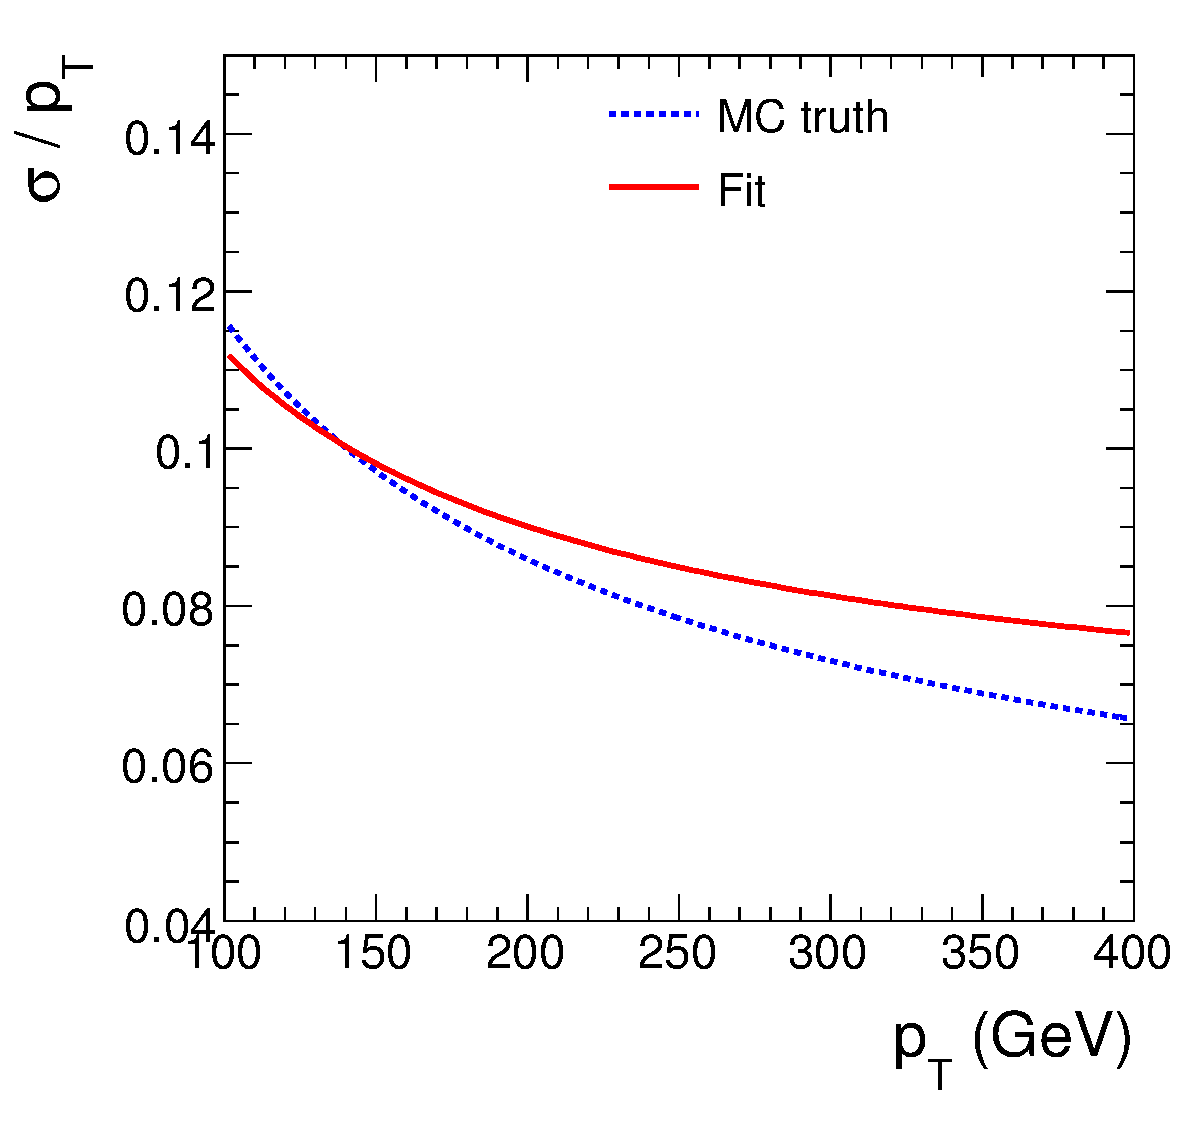
\includegraphics[width=0.45\textwidth]{figures/resFit_PtDependentSigma}
  \caption{Bias due to additional jet activity: \pt dependent $\sigma$}
  \label{fig:ResFit:QCDMC:AddJetAct:Fit}
\end{figure}

In the following Section~\ref{sec:ResFit:QCDMC:Extrapolation}, a method is proposed to correct the resolution
measurement for the effects of additional jet activity.
